\imtnechapitre{Contexte}
\setcounter{section}{0}
\section{Présentation Générale de l'organisation}\cite{infoAfnic}
Née en 1997, l’AFNIC est l’Association Française pour le Nommage Internet en Coopération.
Depuis son origine, elle assure la gestion du registre des noms de domaine en France (plus de 4 millions de noms de domaine en .fr à ce jour), en lien avec l’ensemble de l’écosystème de l’internet en France.
Parce que le .fr est un bien public, le rôle de l’AFNIC s’inscrit dans une mission d’intérêt général et d’opérateur de service essentiel qui consiste à contribuer au quotidien :
\begin{itemize}
    \item A un internet sûr et stable ;
    \item Ouvert aux innovations ;
    \item Où la communauté internet française joue un rôle de premier plan.
\end{itemize}

Outre le .fr, l’AFNIC opère également des extensions pour certains territoires ultramarins (comme le .re depuis 2001 pour l’Ile de la Réunion), et depuis 2014 elle est opérateur technique de nouvelles extensions personnalisées (gTLD). Avec des solutions techniques de registre et AFNIC Conseil, l’association a développé une gamme complète pour accompagner les marques et les territoires qui souhaitent se doter de leur propre extension.

Avec une expertise reconnue dans les infrastructures sous-jacentes de l’internet et notamment le DNS (système des noms de domaine), l’AFNIC prend part à la gouvernance mondiale de l’internet, pour définir les règles et les standards de demain.
Association à but non lucratif, l’AFNIC s’est dotée d’une gouvernance multipartite associant toutes les parties prenantes de l’internet en France : pouvoirs publics, utilisateurs et secteur
privé.
Pour défendre l’intérêt général, l’AFNIC protège son indépendance. Elle ne reçoit aucune subvention de fonctionnement, et œuvre comme une PME (effectif de 91 salariés). Le financement de l’activité est entièrement assuré par la mise à disposition de ses prestations.

\section{Ses Membres}
L’AFNIC étant une association, elle est composée de différents membres :
\begin{itemize}
    \item Des représentants des pouvoirs publics
    \item Des bureaux d’enregistrement 
    \item Des personnes morales (associations d’utilisateurs, etc.)
    \item Des personnes physiques (particuliers)
    \item Des associations/organisation nationales ou internationales
\end{itemize}
\vspace{10pt}
Ces membres sont séparés en trois groupes distincts :

\begin{itemize}
    \item Les bureaux d’enregistrement
    \item Les membres utilisateurs (personnes morales ou particuliers)
    \item Les membres correspondants (Collège International) 
\end{itemize}

\section{Ses Missions}
Les missions de l’AFNIC (telles que définies dans ses statuts) ont globalement pour but de favoriser le développement de l’internet en France.
Plus précisément, ses responsabilités sont :
\begin{itemize}
    \item L’Attribution et la Gestion les noms de domaines dont elle est responsable.
    \item Le transfert (au plan National et International) de ses connaissances et de son savoir faire
    \item Le soutiens au développement d’internet, à la formation et à la sensibilisation à ses usages
    \item Toute autre mission qui lui aura été confiée par les pouvoirs publics dans le cadre de la gestion de l’Internet.
\end{itemize}
L’AFNIC doit aussi reverser 90 \verb|%| des bénéfices de la gestion du .fr à sa Fondation AFNIC pour la solidarité numérique.
Du fait de sa position entre Fournisseurs d’Accès Internet (FAI), Utilisateurs et Autorités Publiques, l’AFNIC est impliqué dans l’évolution de la gouvernance et gestion d’internet au niveau international. Plus précisément, elle :
\begin{itemize}
    \item Participe à la gouvernance globale de l'internet (\GLS{icann}, \GLS{centr}, \GLS{wsis}).
    \item Introduire de nouveaux standards et services (\GLS{ietf}, \GLS{ripencc}).
    \item Transmettre des connaissances et savoir-faire (Collège International de l’AFNIC).
\end{itemize}

\todo{Infos RH, CSE, RSE, etc}

\section{Politique RH et RSE}
L'Afnic a un rythme de travail plutôt spécial, au lieu de travailler 35h en 5 jours, tous les employés travaillent en format 32h en 4 jours (ou 3 jours + 2 demi-journées) sans horaires d'arrivée et de départ fixes (certains préfèrent commencer a 7h et finir a 16h pour éviter les embouteillages et profiter de la fin d'après-midi et d'autres préfèrent faire 10h-19h).
En plus de cela, les employés prennent en général 1 jour de télétravail par semaine.
Cela permet une flexibilité du travail bien plus importante que des horaires de travail classique.




\begin{figure}[ht]
  \noindent
  \begin{minipage}{.6\textwidth}
Pour ce qui est de sa politique RSE, l’Afnic s’est engagée dans la convention signée avec l'Etat en juillet 2012 à évaluer son emprunte carbone à publier les résultats de son Bilan Carbone tous les 3 ans.
    
Cette convention a été renouvelle en 2022 avec quelques changements, l'AFNIC "s'engage à réaliser, au minimum tous les deux ans un bilan carbone" et elle "s'engage à ateindre la neutralité carbone de ses activités à travers la mise en place d'un plan de réduction des Gaz à effet de serre (PRGES) et une politique de compensation carbone.
\cite{conventionAfnic2022}
  \end{minipage}
  \hfill
  \begin{minipage}{.35\textwidth}
    \centering
      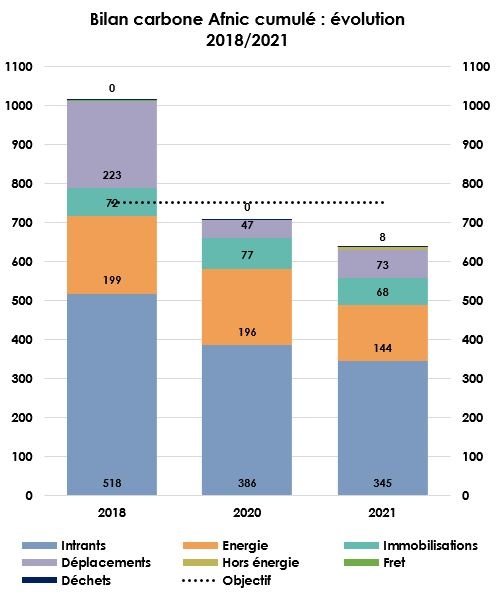
\includegraphics[width=\textwidth]{paper/figures/EvolutionCarbone}
      \caption{Evolution du bilan carbone de l'Afnic}
      \label{fig:evolutionCarbone}
  \end{minipage}
\end{figure}


\section{Qu'est-ce que le DNS}
Le DNS ou Domain Name System (Système de Nom de Domaine en français) est une partie critique au fonctionnement d’internet comme on le connais aujourd’hui.

Son usage principal est de transformer un Nom de Domaine (voir image en dessous) en une adresse IP qui est utilisable pour la transmission.

\begin{figure}[htbp]
  \centering
  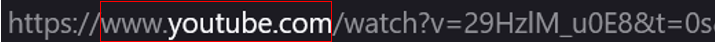
\includegraphics[width=\textwidth]{paper/figures/domainName}
  \caption{Nom de domaine}
  \label{fig:domainName}
\end{figure}

Pour cela, lorsque l’on essaye d’accéder à un site internet (par exemple www.afnic.fr), l’ordinateur envoie une requête dns a son résolveur dns (1).
Ensuite il y a deux cas possibles :

Soit le résolveur n’a pas le Nom de Domaine que l’on demande en mémoire, dans ce cas il doit le trouver de manière récursive.

Il commence par demander aux "\glspl{rootserver}" (2) qui le redirige vers les \glspl{autoritativeserver} sur le \GLSpl{tld} en question. (3)

Ensuite il demande a ces serveurs (4), qui le redirigent vers les \glspl{autoritativeserver} sur la partie suivante du nom de domaine (afnic.fr dans notre cas). (5)

Et il continue jusqu’à trouver le \gls{autoritativeserver} sur le nom qui lui répondra l’adresse ip correspondante. (6)(7)

Finalement une fois que le résolveur connais l'adresse IP corespondant au Nom de Domaine, il la renvois au client (8) qui peut finalement accéder au service souhaité (9)

\begin{figure}[htbp]
  \centering
  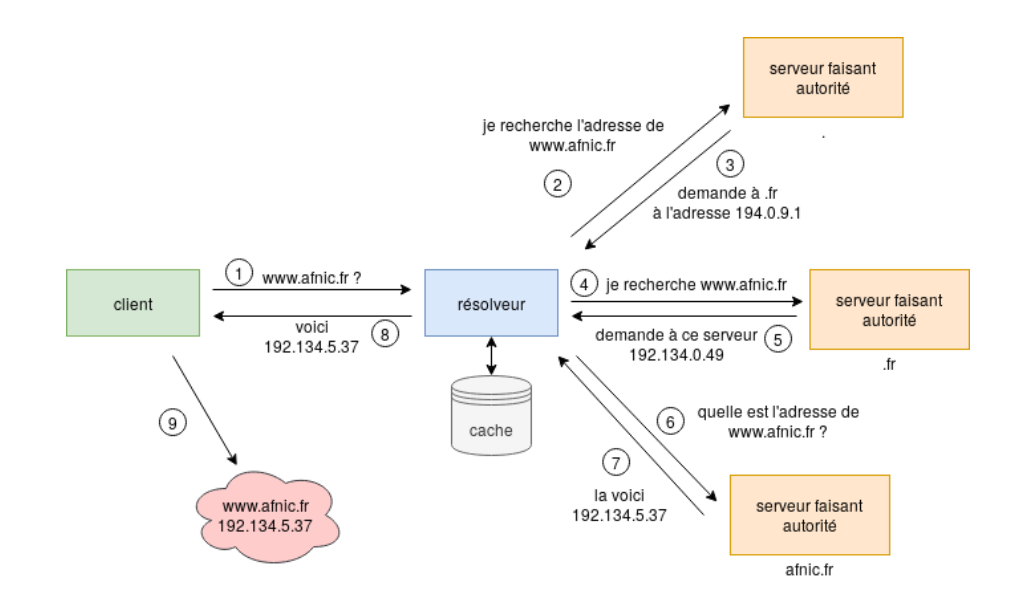
\includegraphics[width=\textwidth]{paper/figures/resolver}
  \caption{Fonctionnement d'un résolveur}
  \label{fig:resolver}
\end{figure}

Si le résolveur connaît déjà l’adresse ip du nom de domaine demandé, il peut répondre directement et sauter les étapes 2 à 7.

Il est aussi possible que le résolveur connaisse déjà une partie du nom de domaine (par exemple on demande zimbra.afnic.fr), dans ce cas il peut directement demander aux serveurs faisant autorité sur la dernière partie commune et sauter les étapes 2 à 5 ce qui divise par deux le nombre de requêtes nécéssaires.

Comme dit plus tôt, un Résolveur fait l’interface entre les clients et les différents serveurs faisant autorité. Ces serveurs intermédiaires ont de nombreux avantages par rapport à faire toutes les requêtes soi-même, principalement au travers de son mécanisme de mémoire (ou Cache).

Premièrement cela réduit le délai de réponse ce qui est très important car le délai des requêtes dns est un des facteurs les plus importants dans la fluidité de navigation sur internet (surtout de nos jours où les connections internet sont de plus en plus rapide). Les résolveurs permettent de réduire le délai de réponse pour plusieurs raisons, la mémoire qui diminue le nombre de requêtes intermédiaires à faire et le fait que les datacenters dans lesquels sont ces serveurs ont des connections internet bien plus rapides que ce qu’un particulier peut obtenir.

Ensuite, cela réduit de façon significative la charge sur les serveurs faisant autorité réduisant les coûts (financiers et environnementaux) de l’infrastructure internet.

Le résolveur dns est généralement assigné en se connectant a un réseau internet, c’est généralement un serveur géré par l’opérateur (Orange, Free, SFR, Bouygues, etc) pour les particuliers et un serveur interne a l’organisation pour les professionnels.

Il existe aussi un certain nombre de résolveur publics (gratuits ou payants) proposant une meilleure vitesse, confidentialité ou même différents services tels que le blocage de publicités, de contenu pornographique ou autre.

Parmi les plus connus on trouve, Google (8.8.8.8), Cloudflare (1.1.1.1), QuadNine (9.9.9.9) et OpenDNS (208.67.222.222).

\section{Un ancien système}
Bien que le protocole DNS soit critique au fonctionnement d’internet, il est très vieux (la RFC 1034 le définissant date de 1987 \cite{dnsRFC}) et il n’est pas vraiment possible de le modifier pour des raisons de compatibilité avec les anciens équipements encore connectés à internet (il n’est pas rare que des équipements critiques soient très anciens notamment dans l’armée, le milieu hospitalier ou l’industrie).

\section{les différentes évolutions}
Sachant qu’il n’est pas possible de modifier le protocole dns directement, d’autres protocoles alternatifs ont été développés pour palier aux différents problèmes qui sont apparus.
\subsection{DoTCP}
Le DoTCP \cite{dotcpRFC} a été le premier protocole alternatif qui est apparu pour palier a la limite de taille dans les réponses DNS, avec l’ajout de l’ipv6, de l’expansion des informations que l’on peut stocker dans le DNS et le développement du DNSSEC, les réponses sont devenues de plus en plus longues et se retrouvent limités par la taille d’un paquet UDP (protocole utilisé par le DNS basic) soit 65,507 bytes.

Le protocole TCP lui permet de séparer un message en plusieurs paquets et permet outre la limite de taille de paquet. Ce protocole a aussi l’avantage de permettre plus de gestion d’erreur et de retransmission en cas de problème sur le réseau.

\subsection{DNSSEC}
Le DNSSEC \cite{dnssecRFC} est une adition au protocole DNS qui permet d’authentifier cryptographiquement la réponse reçue afin d’être sûr qu’elle a bien été renvoyée par le serveur ayant autorité et non par un tiers malicieux.
Cette évolution repose généralement sur les autres protocoles permétant de plus grandes réponses DNS dû a la taille des signatures cryptographiques.

\subsection{DoT}
Le protocole DoT \cite{dotRFC} (DNS over TLS) permet de chiffrer les requêtes DNS via chiffrement TLS (même méthode qu’utilisé pour chiffrer les requêtes http en https).

C'est le premier protocole permétant d’empêcher les intermédiaires (notamment l’opérateur internet ou simplement quelqu’un sur le même réseau) de pouvoir voir tout le trafic dns et donc tous les sites accédés, cependant cela a pour coût la rapidité car l’ajout d’une couche de chiffrement rend la requête plus lourde a traiter pour le client et le serveur.

\subsection{DoH}
Finalement le DoH \cite{dohRFC} (DNS over Https) permet de faire des requêtes dns en passant par le protocole https ce qui les rend presque indistinguables du trafic html classique et est donc très difficile a bloquer par des pare-feu ou autre outil de contrôle (il est facile de bloquer le DoT et donc de forcer l’utilisateur à utiliser d’autres protocoles non privés). 
